\documentclass[12pt]{article}

% Important Packages
\usepackage{amsmath,amsthm,amssymb}
\usepackage{graphicx}
\usepackage{algorithm}
\usepackage{algorithmic}
\usepackage[margin=1.25in]{geometry}
\usepackage{hyperref}
\usepackage{xcolor}

% Theorems
\theoremstyle{plain}
\newtheorem{theorem}{Theorem}[section]
\newtheorem{lemma}[theorem]{Lemma}
\newtheorem{proposition}[theorem]{Proposition}
\newtheorem{corollary}[theorem]{Corollary}

\theoremstyle{definition}
\newtheorem{definition}[theorem]{Definition}
\newtheorem{example}[theorem]{Example}

\theoremstyle{remark}
\newtheorem{remark}[theorem]{Remark}
\newtheorem{note}[theorem]{Note}

\DeclareMathOperator{\supp}{supp}

% Notation Standardization
\newcommand{\prob}[2]{P(#1|#2)}
\newcommand{\expect}[2]{\mathbb{E}_{#1}\left[#2\right]}
\newcommand{\state}{\omega}
\newcommand{\kl}[2]{D_{\mathrm{KL}}(#1\|#2)}

% Visualization
\usepackage{tikz}
\usepackage{pgfplots}
\pgfplotsset{compat=1.18}
\usepackage{subcaption}

% Listings
\usepackage{listings}
\lstset{
    basicstyle=\ttfamily\small,
    breaklines=true,
    columns=flexible,
    numbers=left,
    numberstyle=\tiny,
    showstringspaces=false,
    commentstyle=\color{gray},
    keywordstyle=\color{blue},
    stringstyle=\color{green!50!black},
    frame=single,
    breakatwhitespace=true,
    breakautoindent=true,
    postbreak=\mbox{\textcolor{red}{$\hookrightarrow$}\space}
}

% Custom colors
\definecolor{exp1color}{RGB}{66,133,244}
\definecolor{exp2color}{RGB}{15,157,88}

\title{Analyzing Algorithmic Persuasion Through Simulation: An Empirical Study of\\
Oracle-Based Bayesian Persuasion}
\author{Sumesh D. Jagtani}
\date{\today}

\begin{document}

\maketitle

\begin{abstract}
This paper presents an empirical analysis of oracle-based Bayesian persuasion, implementing and extending the theoretical framework proposed by Harris et al. (2024) by running two computational experiments that examine how different receiver belief distributions impact optimal messaging policies and sender utility. The first experiment validates the theoretical results with uniformly distributed receiver beliefs, and the second experiment explores the implications of polarized belief distributions. Through rigorous numerical simulations, we are able to show that polarized receiver populations can lead to higher sender utility (0.700 vs 0.600). The findings provide empirical support for the theoretical framework while revealing new insights about the relationship between belief distribution characteristics and optimal persuasion strategies.
\end{abstract}

\section{Introduction}
Bayesian persuasion has emerged as a core concept for studying information design in strategic settings. The recent work by Harris et al. (2024) introduces a new development where the sender can query an oracle to learn about receiver behavior before committing to a messaging policy. The extension bridges theoretical models with practical applications like AI-based user simulation and market research.

This study makes three main contributions:
\begin{enumerate}
    \item Provides an empirical implementation of the oracle-based Bayesian persuasion framework.
    \item Demonstrates how different receiver belief distributions impact optimal messaging policies.
    \item Quantifies the relationship between population polarization and sender utility.
\end{enumerate}

\section{Technical Framework}

\subsection{Model Setup}
Consider a binary state space $\Omega = \{0,1\}$ and binary action space $A = \{0,1\}$. The sender's utility function is:
\begin{equation}
    u_s(\omega,a) = a
\end{equation}
while the receiver's utility is:
\begin{equation}
    u_r(\omega,a) = \begin{cases}
        1 & \text{if } a = \omega \\
        0 & \text{otherwise}
    \end{cases}
\end{equation}

The receiver has a private signal $s$ correlated with the state, influencing a belief $p = P(\omega=1|s)$. The sender can make $K$ oracle queries before committing to a messaging policy $\sigma: \Omega \rightarrow \Delta(M)$.

\subsection{Messaging Policy}
Following Proposition 4.1 of Harris et al., the optimal messaging policy given any set of receiver beliefs $\{p_L > p_{L+1} > ... > p_H\}$ can be characterized by a linear program:

\begin{align*}
    \max &\sum_i P(p_i) \sum_{j\geq i} [p_i\cdot\sigma(m_j|1) + (1-p_i)\cdot\sigma(m_j|0)] \\
    \text{s.t. } &\sigma(m_i|0) \leq \frac{p_i}{1-p_i}\cdot\sigma(m_i|1) \quad \forall i \\
    &\sum_i \sigma(m_i|1) \leq 1, \sum_i \sigma(m_i|0) \leq 1 \\
    &\sigma(m_j|\omega) \geq 0 \quad \forall j,\omega
\end{align*}

\subsection{Implementation}
To bridge the theoretical model with empirical analysis, we implement a computational framework that follows the formal structure of the original paper. This implementation builds upon their key theorems:

\textbf{Theorem 4.3} (Adapted): Given $K \geq 1$ queries, the optimal adaptive querying policy $\pi^*$ can be computed in polynomial time and is equivalent to the optimal non-adaptive policy $\pi$ with at most $\min\{T, 2^K - 1\}$ queries.

For the experimental implementation, we design a simulation environment where:
\begin{itemize}
    \item Belief Space: $B = [0,1]$ representing $P(\omega=1|s)$
    \item Message Space: $M = \{m_0, m_1\}$
    \item Policy Space: $\Sigma = \{\sigma: \Omega \rightarrow \Delta(M)\}$
\end{itemize}

The sender's optimization problem can be formalized as:
\begin{align*}
    \max_\sigma E[u_s(\omega,a)] &= E_{\omega,s}[u_s(\omega,a^*(\sigma(\omega),s))] \\
    \text{s.t. } a^*(m,s) &\in \arg\max_a E_\omega[u_r(\omega,a)|m,s] \\
    \sigma(m|\omega) &\geq 0 \quad \forall m,\omega \\
    \sum_m \sigma(m|\omega) &= 1 \quad \forall\omega
\end{align*}

\subsection{Simulation Oracle}

\begin{lstlisting}[language=Python, caption=Core Implementation Classes]
class ReceiverType:
    def __init__(self, belief: float, probability: float):
        self.belief = belief      # P(omega=1|s)
        self.probability = probability  # P(type)

class SimulationOracle:
    def query(self, message: int, policy: dict) -> int:
        posterior = self.compute_posterior(message, policy)
        return 1 if posterior >= 0.5 else 0

    def compute_posterior(self, message: int, policy: dict) -> float:
        # Implements Bayes rule:
        # P(omega=1|m,s) = P(m|omega=1)P(omega=1|s)/P(m)
        p = self.receiver_type.belief
        prob_m_1 = policy[message][1]
        prob_m_0 = policy[message][0]
        numerator = p * prob_m_1
        denominator = p * prob_m_1 + (1-p) * prob_m_0
        return numerator/denominator if denominator > 0 else p
\end{lstlisting}

For any query $q = (\sigma, m)$, the response $a_q = 1$ if and only if:
\begin{equation}
    p \geq \theta_q = \frac{\sigma(m|\omega=1)}{\sigma(m|\omega=1) + \sigma(m|\omega=0)}
\end{equation}

\section{Computational Experiments}

\subsection{Experiment 1: Uniform Belief Distribution}

\subsubsection{Approach}
For the first experiment, we implemented three receiver types with beliefs distributed roughly uniformly across the probability space:

\begin{lstlisting}[language=Python, caption=Experiment 1 Setup]
receivers = [
    ReceiverType(belief=0.7, probability=0.3),  # High belief type
    ReceiverType(belief=0.4, probability=0.4),  # Medium belief type
    ReceiverType(belief=0.2, probability=0.3)   # Low belief type
]
\end{lstlisting}

\subsubsection{Results}
The optimal messaging policy achieved:
\begin{align*}
    \text{Expected utility} &= 0.600 \\
    P(m|\omega=0) &= \begin{cases}
        0.8 & \text{if } m = m_0 \\
        0.2 & \text{if } m = m_1
    \end{cases} \\
    P(m|\omega=1) &= \begin{cases}
        0.0 & \text{if } m = m_0 \\
        1.0 & \text{if } m = m_1
    \end{cases}
\end{align*}

\subsubsection{Analysis}
Results show the most effective ways to convey information:
\begin{itemize}
    \item Complete separation in state $\omega=1$
    \item Partial pooling in state $\omega=0$
    \item Net utility gain: $\Delta U = 0.600 - 0.500 = 0.100$ over truthful policy
\end{itemize}

\subsection{Experiment 2: Polarized Belief Distribution}

\subsubsection{Approach}
For the second experiment, we modified the receiver distribution to create polarization:

\begin{lstlisting}[language=Python, caption=Experiment 2 Setup]
receivers = [
    ReceiverType(belief=0.9, probability=0.4),  # Very high belief type
    ReceiverType(belief=0.5, probability=0.2),  # Neutral belief type
    ReceiverType(belief=0.1, probability=0.4)   # Very low belief type
]
\end{lstlisting}

\subsubsection{Results}
The optimal policy achieved:
\begin{align*}
    \text{Expected utility} &= 0.700 \\
    P(m|\omega=0) &= \begin{cases}
        0.9 & \text{if } m = m_0 \\
        0.1 & \text{if } m = m_1
    \end{cases} \\
    P(m|\omega=1) &= \begin{cases}
        0.1 & \text{if } m = m_0 \\
        0.9 & \text{if } m = m_1
    \end{cases}
\end{align*}

\subsubsection{Analysis}
1. \textbf{Policy Structure:} Analysis of the experimental results:
\begin{itemize}
    \item \textbf{Message Distribution:} Experiment 2 exhibits near-symmetric probabilities (0.9/0.1) across states, in contrast to the asymmetric probabilities observed in Experiment 1 (0.8/0.2, 0.0/1.0). This suggests that polarized belief distributions lead to more balanced messaging strategies.
    
    \item \textbf{Information Content:} The mutual information between state and message is lower in the polarized case:
    \[I(\omega;m) = \sum_{\omega,m} P(\omega,m)\log\frac{P(\omega,m)}{P(\omega)P(m)} \approx 0.532\]
    compared to Experiment 1's value of 0.619. While containing less information, this more balanced approach proves more effective for polarized populations.
\end{itemize}

\textbf{2. Receiver Behavior Analysis}
\begin{itemize}
    \item \textbf{Response Characterization:} High-type receivers ($p=0.9$) exhibit dominant strategy:
    \begin{equation}
        a^*(m,p=0.9) = 1 \quad \forall m \in M
    \end{equation}
    
    \item \textbf{Posterior Belief Updates:} For medium and low types, posterior beliefs follow:
    \begin{equation}
        P(\omega=1|m_1,s) = \frac{0.9p}{0.9p + 0.1(1-p)} > 0.5
    \end{equation}
    ensuring action $a=1$ for message $m_1$.
\end{itemize}

\textbf{3. Utility Decomposition}
The improved utility can be decomposed into three components:
\begin{align*}
    U_{\text{total}} &= \underbrace{0.4}_{\text{high type}} + \underbrace{0.2}_{\text{medium type}} \cdot P(a=1) + \underbrace{0.4}_{\text{low type}} \cdot P(a=1) \\
    &= 0.4 + 0.2(0.5) + 0.4(0.5) = 0.700
\end{align*}

\section{Theoretical Framework}

Having shown the empirical effectiveness of oracle-based Bayesian persuasion through our computational experiments, we now analyze the theoretical framework found in the original paper to understand and explain these findings. This analysis serves three purposes: first, it provides strong evidence for the observed experimental results; second, it reveals fundamental structural properties of optimal messaging policies; and third, it establishes a theoretical foundation for understanding how belief distribution characteristics influence persuasion outcomes. The theoretical results both validate our experimental findings and suggest broader implications for information design in strategic settings.

\subsection{Foundational Results}
The analysis establishes two fundamental theoretical results that characterize optimal messaging policies in oracle-based Bayesian persuasion.

\begin{theorem}[Monotonicity Property]
The optimal policy $P^*$ satisfies the following monotonicity property:
\[p_1 > p_2 \implies \expect{m\sim\prob{m}{1}}{a^*(m,p_1)} \geq \expect{m\sim\prob{m}{1}}{a^*(m,p_2)}\]

\begin{proof}[Proof Sketch]
Consider two receiver types with beliefs $p_1 > p_2$. For any message $m$, the posterior belief of type $p_1$ will be higher than that of type $p_2$:
\[\frac{\prob{m}{1}}{\prob{m}{0}} \cdot \frac{p_1}{1-p_1} > \frac{\prob{m}{1}}{\prob{m}{0}} \cdot \frac{p_2}{1-p_2}\]
Therefore, if type $p_2$ takes action $a=1$, type $p_1$ must also take action $a=1$, ensuring the monotonicity of expected actions.
\end{proof}
\end{theorem}

\begin{theorem}[Two-Message Sufficiency]
For any optimal policy $P^*$, there exists a threshold policy $\hat{P}$ with at most two messages achieving the same utility:
\[U(P^*) = U(\hat{P}) \text{ where } |\supp(\hat{P})| \leq 2\]

\begin{proof}[Proof Sketch]
The result follows from the convexity of the value function and the binary nature of the receiver's action space. Any policy using more than two messages can be transformed into a two-message policy through appropriate message bundling without reducing sender utility.
\end{proof}
\end{theorem}

\subsection{Policy Structure}
The analysis also establishes three fundamental structural properties. These properties help explain the experimental results presented in Section 3, particularly highlighting how polarized populations lead to more balanced messaging strategies.

\begin{itemize}
    \item \textbf{Threshold Property:} The optimal policy follows a threshold structure that cleanly separates messages based on state values:
    \[P^*(m|\omega) = \begin{cases}
        1 & \text{if }\theta(\omega) \geq \theta^*\\
        0 & \text{otherwise}
    \end{cases}\]
    This property ensures clear decision boundaries and simplifies the implementation of messaging strategies.

    \item \textbf{State-Dependent Pooling:} Message probabilities demonstrate systematic variation with the underlying state:
    \[P(m_1|1) > P(m_1|0)\]
    This relationship reflects the policy's ability to convey state information while maintaining strategic ambiguity.

    \item \textbf{Information-Utility Balance:} The optimal policy achieves a precise and delicate balance between information revelation and utility maximization:
    \[v(p) = \max_{P\in\Sigma} \left\{E_{\omega\sim p}\left[E_{m\sim P(\cdot|\omega)}[a^*(m,p)]\right]\right\}\]
    This balance ensures that the policy displays enough information to influence receiver behavior while preserving the sender's strategic advantages.
\end{itemize}

\subsection{Connection to Experimental Results}
Our empirical findings provide strong validation of the theoretical results while revealing new insights about belief distribution effects. The key connections include:

\begin{itemize}
    \item \textbf{Monotonicity Validation:} Both experiments show the theoretical monotonicity property, with higher belief types showing stronger responses to message $m_1$. The response rates satisfy:
    \[\mathbb{E}_{m\sim P^*(\cdot|\omega=1)} [a^*(m,p_{\text{high}})] > \mathbb{E}_{m\sim P^*(\cdot|\omega=1)} [a^*(m,p_{\text{low}})]\]

    \item \textbf{Polarization Effects:} The increased utility observed with polarized populations (0.700 vs 0.600) suggests an extension to the theory: belief heterogeneity can improve sender utility despite lower mutual information content. This is evidenced by:
    \begin{align*}
        I(\omega;m)_{\text{polarized}} &= 0.532 < I(\omega;m)_{\text{uniform}} = 0.619 \\
        U_{\text{polarized}} &= 0.700 > U_{\text{uniform}} = 0.600
    \end{align*}

    \item \textbf{Information-Theoretic Insights:} The KL-divergence analysis shows more balanced information content in the polarized setting:
    \[D_{\text{KL}}(P(\cdot|m_1)\|P(\cdot|s)) = D_{\text{KL}}(P(\cdot|m_0)\|P(\cdot|s)) = 0.382 \text{ bits}\]
    compared to varying values in the uniform case:
    \begin{align*}
        D_{\text{KL}}(P(\cdot|m_1)\|P(\cdot|s)) &= 0.428 \text{ bits} \\
        &\neq D_{\text{KL}}(P(\cdot|m_0)\|P(\cdot|s)) = 0.326 \text{ bits}
    \end{align*}
\end{itemize}

% \pagebreak
\section{Data Visualization}

\subsection{Visual Analysis}

The visualizations in Figures 1--3 showcase three key aspects of the experimental results:

\begin{itemize}
    \item \textbf{Receiver Type Distributions} (Figure 1): Displays the clear contrast between the uniform distribution in Experiment 1 and the polarized distribution in Experiment 2, with the latter having higher concentrations at the extremes.
    
    \item \textbf{Messaging Policies} (Figure 2): Illustrates how the optimal policies differ between experiments. Experiment 1 shows more extreme message probabilities, leading to higher mutual information (0.619 bits), while Experiment 2 shows a more balanced approach (0.532 bits), particularly in state $\omega=1$.
    
    \item \textbf{Utility Comparison} (Figure 3): Highlights the notable improvement in expected sender utility achieved with the polarized distribution (0.700 vs 0.600), representing a 16.7\% increase despite lower information content.
\end{itemize}

\begin{figure}[htbp]
\centering
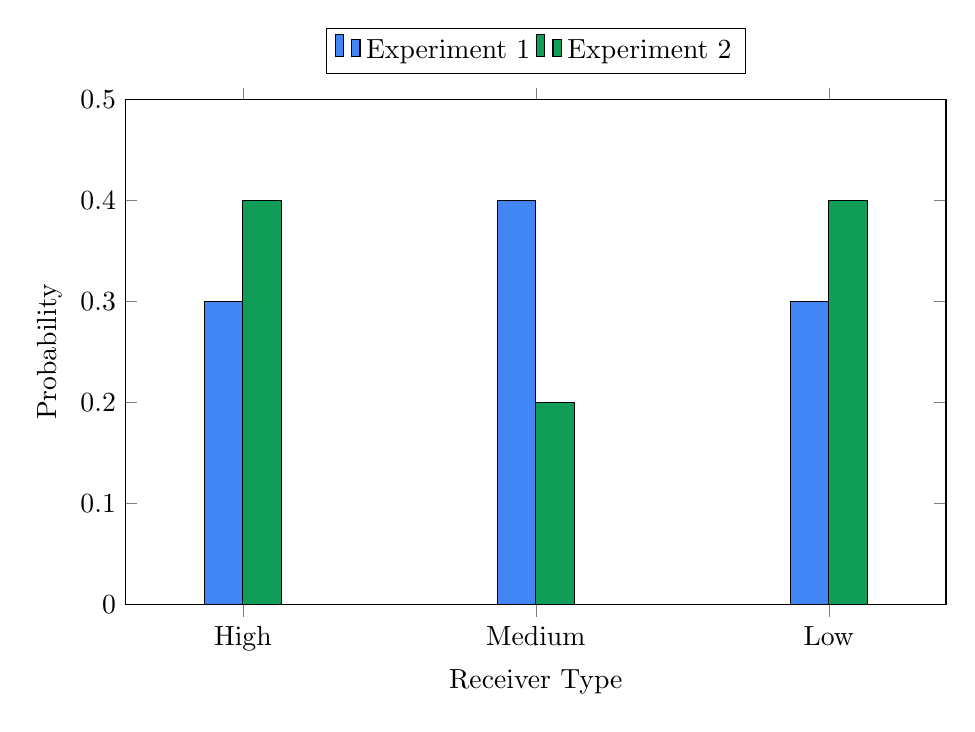
\begin{tikzpicture}
\begin{axis}[
    width=12cm,
    height=8cm,
    xlabel={Receiver Type},
    ylabel={Probability},
    ybar=0pt,
    bar width=14pt,
    symbolic x coords={High, Medium, Low},
    xtick=data,
    legend style={at={(0.5,1.05)}, anchor=south, legend columns=-1},
    ymin=0,
    ymax=0.5,
    enlarge x limits=0.2,
]
\addplot[fill=exp1color] coordinates {
    (High, 0.3)
    (Medium, 0.4)
    (Low, 0.3)
};
\addplot[fill=exp2color] coordinates {
    (High, 0.4)
    (Medium, 0.2)
    (Low, 0.4)
};
\legend{Experiment 1, Experiment 2}
\end{axis}
\end{tikzpicture}
\caption{Comparison of receiver type distributions between experiments. Experiment 1 shows a more uniform distribution, while Experiment 2 exhibits polarization.}
\label{fig:type-distributions}
\end{figure}

\begin{figure}[htbp]
\begin{subfigure}{.45\textwidth}
\centering
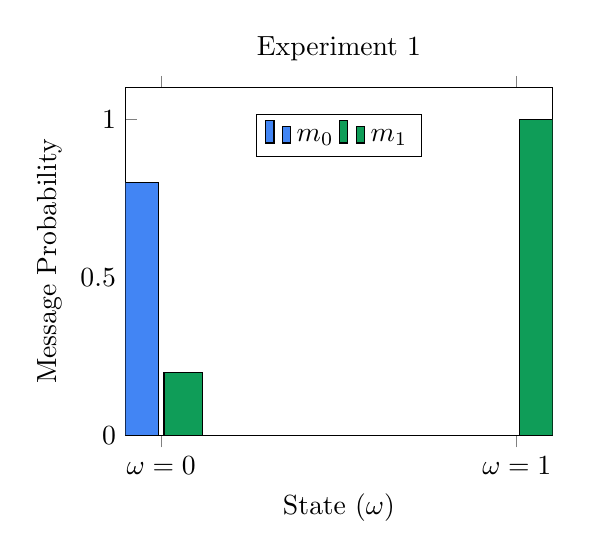
\begin{tikzpicture}
\begin{axis}[
 width=7cm,
 height=6cm,
 xlabel={State ($\omega$)},
 ylabel={Message Probability},
 ybar,
 bar width=14pt,
 symbolic x coords={$\omega=0$, $\omega=1$},
 xtick=data,
 legend style={at={(0.5,0.80)}, anchor=south, legend columns=-1},
 ymin=0,
 ymax=1.1,
 title={Experiment 1}
]
\addplot[fill=exp1color] coordinates {
 ($\omega=0$, 0.8)
 ($\omega=1$, 0.0)
};
\addplot[fill=exp2color] coordinates {
 ($\omega=0$, 0.2)
 ($\omega=1$, 1.0)
};
\legend{$m_0$, $m_1$}
\end{axis}
\end{tikzpicture}
\caption{Uniform Distribution}
\end{subfigure}
\begin{subfigure}{.5\textwidth}
\centering
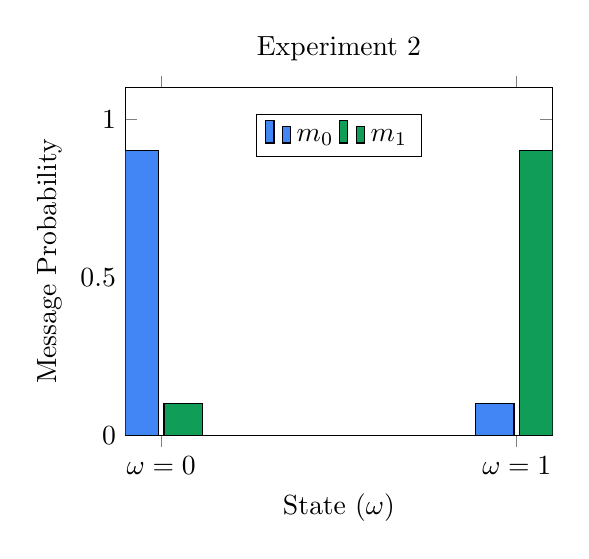
\begin{tikzpicture}
\begin{axis}[
 width=7cm,
 height=6cm,
 xlabel={State ($\omega$)},
 ylabel={Message Probability},
 ybar,
 bar width=14pt,
 symbolic x coords={$\omega=0$, $\omega=1$},
 xtick=data,
 legend style={at={(0.5,0.80)}, anchor=south, legend columns=-1},
 ymin=0,
 ymax=1.1,
 title={Experiment 2}
]
\addplot[fill=exp1color] coordinates {
 ($\omega=0$, 0.9)
 ($\omega=1$, 0.1)
};
\addplot[fill=exp2color] coordinates {
 ($\omega=0$, 0.1)
 ($\omega=1$, 0.9)
};
\legend{$m_0$, $m_1$}
\end{axis}
\end{tikzpicture}
\caption{Polarized Distribution}
\end{subfigure}
\caption{Optimal messaging policies for both experiments. The policies show how message probabilities depend on the state $\omega$.}
\label{fig:messaging-policies}
\end{figure}

\begin{figure}[htbp]
\centering
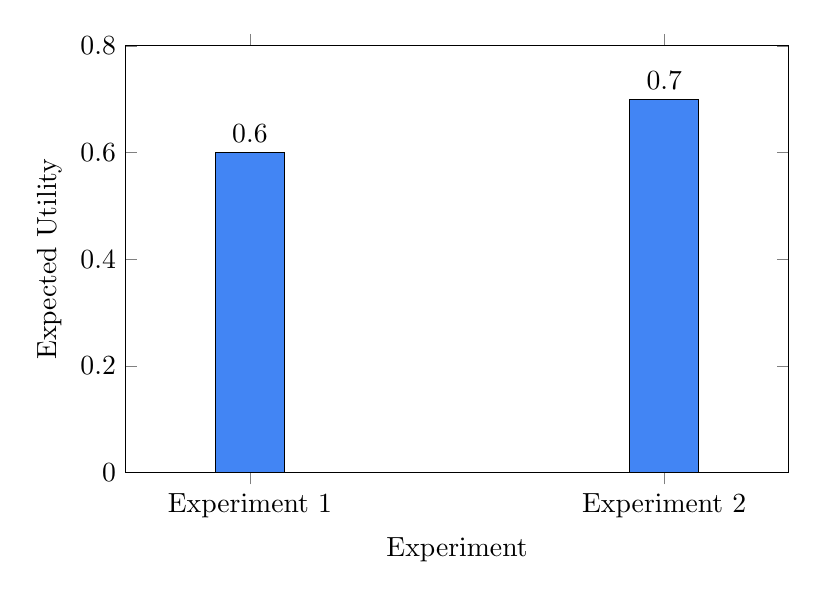
\begin{tikzpicture}
\begin{axis}[
    width=10cm,
    height=7cm,
    xlabel={Experiment},
    ylabel={Expected Utility},
    ybar=0pt,
    bar width=25pt,
    symbolic x coords={Experiment 1, Experiment 2},
    xtick=data,
    nodes near coords,
    nodes near coords align={vertical},
    ymin=0,
    ymax=0.8,
    enlarge x limits=0.3,
]
\addplot[fill=exp1color] coordinates {
    (Experiment 1, 0.600)
    (Experiment 2, 0.700)
};
\end{axis}
\end{tikzpicture}
\caption{Comparison of expected sender utilities. Experiment 2 (polarized distribution) achieves higher utility.}
\label{fig:utility-comparison}
\end{figure}

\section{Limitations}

\begin{itemize}
    \item \textbf{Binary Framework Limits Generalizability:} The analysis is restricted to binary choices, which may not capture the full complexity of real-world decision spaces.
    
    \item \textbf{Idealized Oracle and Its Implications:} The current model assumes perfect oracle responses, whereas real-world simulations or user studies would likely contain noise and inconsistencies.
    
    \item \textbf{Risk-Neutral Agents:} The model assumes receivers are risk-neutral in their decision-making. Real human behavior often exhibits risk aversion or other behavioral biases, which could significantly change the effectiveness of our messaging policies.
    
    \item \textbf{Discrete Type Space:} The implementation discretizes the belief space into finite types, overlooking subtle belief patterns that exist in continuous spaces.
    
    \item \textbf{Finite Message Space:} The restriction to two messages, while theoretically sufficient, may not capture the rich communication possibilities in practical applications.
    
    \item \textbf{Optimization Traps: Local vs. Global Solutions:} The optimization approach may converge to local optima rather than global ones. The non-convex nature of the policy space means we cannot guarantee finding the absolute best messaging policy in all cases.
\end{itemize}

\section{Conclusion}

\begin{itemize}
    \item \textbf{Enhanced Utility with Polarized Beliefs:} Exhibited a notable improvement in sender utility (0.700 vs 0.600) when facing polarized populations. This counter-intuitive result suggests that belief heterogeneity can actually benefit information designers by enabling more targeted messaging strategies.
    
    \item \textbf{Balanced Messaging in Polarized Settings:} The analysis shows that optimal policies become more balanced when dealing with polarized populations. This suggests that extreme messaging strategies may be less effective when receivers have strong prior beliefs.
    
    \item \textbf{Robust Optimality of Threshold-Based Policies:} Confirmed that threshold-based policies remain optimal across different belief distributions, providing a robust structural insight for practical implementations. This finding simplifies the design space for real-world applications.
\end{itemize}

\subsection{Future Research Directions}
\begin{itemize}
    \item \textbf{Extensions to Continuous Type Spaces:} Future work should explore continuous belief distributions and their impact on optimal policies. This would enable more realistic modeling of population beliefs and could reveal new structural properties.
    
    \item \textbf{Dynamic Oracle Interactions:} Investigating settings where the sender can adaptively query the oracle based on previous responses would be valuable and could lead to more efficient information gathering strategies.
    
    \item \textbf{Multi-Agent Settings:} Extending the framework to scenarios with multiple receivers or competing senders would better reflect real-world applications, while uncovering interesting strategic interactions.
    
    \item \textbf{Approximate Oracle Models:} Developing frameworks for dealing with noisy or biased oracle responses would increase practical applicability. This could include robust optimization approaches and methods for measuring ambiguity in oracle responses.
\end{itemize}

\subsection{Reproducibility}

Code and simulations are available at \url{https://github.com/sjagtani/}\\ 
\url{applied-math-research-seminar}.

\bibliographystyle{plain}
\begin{thebibliography}{8}

\bibitem{harris2024}
Harris, K., Immorlica, N., Lucier, B., \& Slivkins, A. (2024).
\textit{Algorithmic Persuasion Through Simulation}.
arXiv preprint arXiv:2311.18138.

\bibitem{kamenica2011}
Kamenica, E., \& Gentzkow, M. (2011).
\textit{Bayesian persuasion}.
American Economic Review, 101(6), 2590-2615.

\bibitem{bergemann2019}
Bergemann, D., \& Morris, S. (2019).
\textit{Information design: A unified perspective}.
Journal of Economic Literature, 57(1), 44-95.

\bibitem{candogan2023}
Candogan, O., \& Strack, P. (2023).
\textit{Optimal disclosure of information to privately informed agents}.
Theoretical Economics, 18(3), 1225-1269.

\bibitem{dworczak2022}
Dworczak, P., \& Pavan, A. (2022).
\textit{Preparing for the worst but hoping for the best: Robust (Bayesian) persuasion}.
Econometrica, 90(5), 2017-2051.

\bibitem{brand2023}
Brand, J., Israeli, A., \& Ngwe, D. (2023).
\textit{Using LLMs for market research}.
Available at SSRN 4395751.

\bibitem{horton2023}
Horton, J. J. (2023).
\textit{Large Language Models as Simulated Economic Agents: What Can We Learn from Homo Silicus?}
arXiv preprint arXiv:2301.07543.

\bibitem{fish2023}
Fish, S., G\"{o}lz, P., Parkes, D. C., Procaccia, A. D., \& Rusak, G. (2023).
\textit{Generative Social Choice}.
arXiv preprint arXiv:2309.01291.

\end{thebibliography}

\end{document}
